\chapter{Constraints}
\section{Definitions}
Any physical system has constraints which limit the motion of parts of the system. They act through forces (forces of constraint). Those forces are unknown and must be obtained through Newton's laws from the effects on other forces.\\
\textbf{Ex.} Normal forces:
\begin{figure}[H]
    \centering
    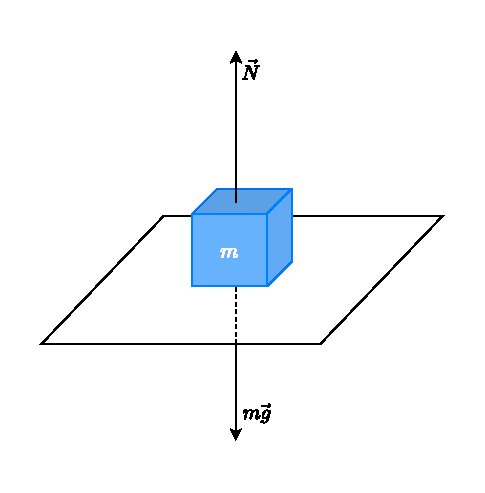
\includegraphics[width=0.5\linewidth]{res/svg/normalforce.drawio}
    \caption{Normal force on a plane}
    \label{fig:image6}
\end{figure}
Let's look deeper with another example. Imagine taking two masses $m_1$ and $m_2$ attached with an inextensible rope through an ideal pulley (massless and frictionless). Also consider the plane frictionless, we get this type of situation:
\begin{figure}[H]
    \centering
    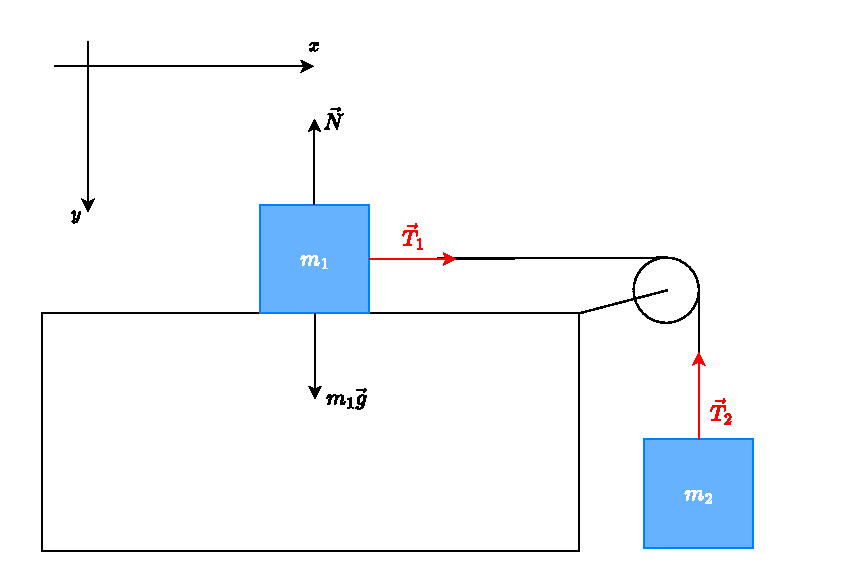
\includegraphics[width=0.6\linewidth]{res/svg/idealpulley.drawio}
    \caption{Normal force on a plane}
    \label{fig:image7}
\end{figure}
The ideal pulley gives us the information that $I\alpha = 0 \Rightarrow T_1 = T_2$. We also know that:
\[a_1 = a_2\]
This is the effect of the inextensible rope which is a \textbf{constraint} for the system. Solving Newton's equations leads to:
\begin{equation}
    \centering
\begin{cases}
T_1=T_2=m_1a \\[8pt]
m_2g -T =m_2a \\[8pt]
\end{cases} \Rightarrow a = \dfrac{m_2}{m_1+m_2}g
\end{equation}
\begin{definition}{Holomonic constraint}
  A constraint is said to be holomonic if it can be expressed as a function:
  \begin{equation}
    f(\vec{r}_1,\vec{r}_2, \,\dots\, ,\vec{r}_n,t) = 0
  \end{equation}
\end{definition}
For the inextensible rope the constraint can be expressed as $\dd{x}=\dd{y}$, but if we choose an appropriate frame of reference the condition can also simply be $x=y$, so the rope is a holomonic constraint such that:
\begin{equation}
    f(x,y)=0 \Rightarrow x-y=0
\end{equation}
If a constraint can be expressed as a function of the velocities it is said to be \textbf{semi-holomonic} and has a form such as:
\begin{equation}
    f(\dvec{r}_1,\dvec{r}_2, \,\dots\, ,\dvec{r}_n,t) = 0
\end{equation}
There are two main types of holomonic constraints:
\begin{itemize}
    \item \textbf{scleromonic} if it \underline{does not} depend on time explicitly \[f(\vec{r}_1,\vec{r}_2, \,\dots\, ,\vec{r}_n) = 0\]
    \item \textbf{rheomonic} if it \underline{does} depend on time explicitly \[f(\vec{r}_1,\vec{r}_2, \,\dots\, ,\vec{r}_n,t) = 0\]
\end{itemize}
A constraint allows us to express any coordinate as a function of the others, so, if we have $N$ particle we should have $3N$ coordinates, but if we have $K$ constraints the actual number of independent coordinates is:
\begin{equation}
    n = 3N-K = \text{dof (degrees of freedom)}
\end{equation}
\section{Virtual displacement}
\begin{definition}{Virtual displacement}
  A virtual displacement is an infinitesimal change in the configuration of the system that results in a change in the particle position compatible with the forces of constraint of the system \underline{at a given time}.
\end{definition}
To explain the difference between a virtual displacement and an actual displacement we can analyze the displacement of a moving object on an inclined plane with the angle changing over time:
\begin{figure}[H]
  \centering
  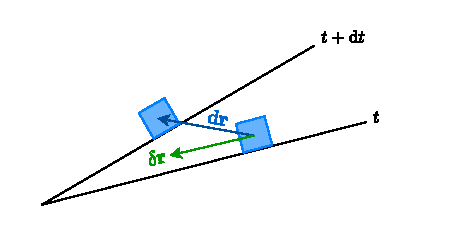
\includegraphics[width=0.5\linewidth]{res/svg/virtualdisplacement.drawio}
  \caption{Displacement and virtual displacement}
  \label{fig:image8}
\end{figure}
Where:
\begin{itemize}
    \item $\delta \vec{r}$ is the virtual displacement
    \item $\dd{\vec{r}}$ is the actual displacement
\end{itemize}
Now consider a system of particles at equilibrium so that:
\begin{equation}
    \vec{F}_i = 0\;\forall i
\end{equation}
The total force is composed of two separated parts:
\begin{itemize}
    \item Applied forces $\vec{F}^{(a)}_i$
    \item Constraint forces $\vec{f}_i$
\end{itemize}
At equilibrium we get:
\begin{equation}
    \begin{split}
      &\bigsum_i \vec{F}_i \cdot \delta \vec{r}_i = 0 \\[8pt]
      &\bigsum_i \brackets{\vec{F}^{(a)}_i + \vec{f}_i} \cdot \delta \vec{r}_i = \bigsum_i \vec{F}^{(a)}_i \cdot \delta \vec{r}_i + \bigsum_i \vec{f}_i \cdot \delta \vec{r}_i = 0
    \end{split}
\end{equation}
Now we consider only system with zero total virtual work, and we get:
\begin{equation}
    \begin{split}
      &\bigsum_i \vec{F}^{(a)}_i \cdot \delta \vec{r}_i + \cancel{\bigsum_i \vec{f}_i \cdot \delta \vec{r}_i} = 0 \\[8pt]
      &\bigsum_i \vec{F}^{(a)}_i \cdot \delta \vec{r}_i = 0
    \end{split}
\end{equation}
The last equation represents the condition of equilibrium for a system such that $\bigsum_i \vec{f}_i \cdot \delta \vec{r}_i = 0$ and is called \textbf{principle of virtual work}.
If the system \underline{is not} at equilibrium then we have:
\begin{equation}
    \vec{F}_i = \dvec{p}_i \Rightarrow \vec{F}_i - \dvec{p}_i = 0
\end{equation}
From which follows:
\begin{equation}
    \bigsum_i \brackets{\vec{F}_i - \dvec{p}_i} \cdot \delta \vec{r}_i = \bigsum_i \brackets{\vec{F}^{(a)}_i + \vec{f}_i - \dvec{p}_i} \cdot \delta \vec{r}_i = 0
\end{equation}
Now if the total virtual work of constraints is 0:
\begin{equation}
    \bigsum_i \brackets{\vec{F}^{(a)}_i - \dvec{p}_i} \cdot \delta \vec{r}_i + \cancel{\bigsum_i \vec{f}_i \cdot \delta \vec{r}_i} = 0
\end{equation}
And we get the so called \textbf{D'Alembert's principle}:
\begin{equation}  \label{D'Alembert_principle}
    \boxed{\bigsum_i \brackets{\vec{F}^{(a)}_i - \dvec{p}_i} \cdot \delta \vec{r}_i = 0}
\end{equation}
Now a problem arises. Since the $\delta \vec{r}_i$ are not independent in these coordinates we need to find a new set of coordinates that makes us able to make all the terms in the sum independent so we can establish that every single term is independently zero.
Those coordinates are called \textbf{generalized coordinates}.\\
Let us now consider only holomonic constraints so we have:
\begin{itemize}
    \item $N$ particles $\Rightarrow$ $3N$ coordinates
    \item $K$ constraints
\end{itemize}
So we actually have $n = 3N-K$ independent coordinates as we stated while talking about constraints in general. So we define the general coordinates:
\begin{equation}
    q_{\alpha}\;\forall\;\alpha = 1, \,\dots\, ,n
\end{equation}
As we stated all the original coordinates must only depend on the $q_{\alpha}$'s and (eventually) on time.
\begin{equation} \label{equations_of_transformation}
    \begin{cases}
        \vec{r}_1 = \vec{r}_1\brackets{q_1, \,\dots\, ,q_n,t}\\[8pt]
        \vec{r}_2 = \vec{r}_2\brackets{q_1, \,\dots\, ,q_n,t}\\[8pt]
         \,\dots\,  \\[8pt]
        \vec{r}_N = \vec{r}_N\brackets{q_1, \,\dots\, ,q_n,t}
    \end{cases}
\end{equation}
These are called the \textbf{equations of transformation}, and they have some properties:
\begin{itemize}
    \item explicitly contain the constraints
    \item can depend on time or not
    \item $q_{\alpha}$'s may not be lengths
    \item $q_{\alpha}$'s may not be grouped in vectors
    \item $q_{\alpha}$'s are scalars
\end{itemize}
An example of the use of generalized coordinates is the use of polar coordinates for the analysis of the pendulum system. In that case there are only 2 coordinates, but there is a constraint on the distance between the mass and the pole of the rotation, so we only have one independent coordinate:
\[q=\theta\]
Obviously it is possible to express general coordinates in terms of regular coordinates:
\begin{equation} \label{inverse_equations_of_transformation}
    \begin{cases}
        q_1 = q_1\brackets{\vec{r}_1, \,\dots\, ,\vec{r}_N,t}\\[8pt]
        q_2 = q_2\brackets{\vec{r}_1, \,\dots\, ,\vec{r}_N,t}\\[8pt]
         \,\dots\,  \\[8pt]
        q_n = q_n\brackets{\vec{r}_1, \,\dots\, ,\vec{r}_N,t}
    \end{cases}
\end{equation}
